\chapter{Finding symmetries using ansätze} \label{ch:ansatze}

Finding symmetries of first order ODE:s is as previously stated different than finding symmetries of higher order models.
For the sake of simplicity, the problem will be shown for scalar explicit ODE:s, or in other words ODE:s on the form
\begin{equation} \label{eq:scalar-explicit-ode}
  \prolongpart{y}{n} = \omega(\prolong{z}{n-1}),
\end{equation}
where \(\prolongpart{y}{n}\) is the \(n\):th derivative in \(x\).
Since \cref{eq:scalar-explicit-ode} is of degree \(n\), the linearized symmetry condition is
\begin{equation} \label{eq:linearized-general-symmetry^ansatze}
  \eval{\prolong{X}{n}(\prolongpart{y}{n} - \omega(\prolong{z}{n-1}))}_{\prolongpart{y}{n} = \omega(\prolong{z}{n-1})} = 0.
\end{equation}
\Cref{eq:linearized-general-symmetry^ansatze} is a partial differential equation (PDE) of degree \(n\) in the functions \(\xi(x, y), \eta(x, y)\).
The highest order jet variable \(\prolongpart{y}{n}\) will not be present anywhere in \cref{eq:linearized-general-symmetry^ansatze} as the evaluation on \cref{eq:scalar-explicit-ode} removes all such dependence.
For an ODE of degree \(n > 1\), jet variables \(\prolongpart{y}{1}, \dots, \prolongpart{y}{n-1}\) will still be present in \cref{eq:linearized-general-symmetry^ansatze}, and since neither \(\xi\) nor \(\eta\) has any dependence on those variables the equation can be decomposed in those variables.
This means that \cref{eq:linearized-general-symmetry^ansatze} will be turned into a system of PDE:s, still of degree \(n\) in the functions \(\xi(x, y), \eta(x, y)\), called the determining equations of the symmetries.
In general, such a system is solvable and thus all symmetries of the systems can be calculated.
Much theory in the literature is built around the assumption that the determining equations exist, and that they (at least in theory) can be solved.

For an ODE of degree \(n = 1\) such a decomposition is not possible, since no jet variables except for \(x\) and \(y\) are present in \cref{eq:linearized-general-symmetry^ansatze}.
Instead, the \enquote{determining equations} is the same equation as the linearized symmetry condition.
The common solution to this problem is to use an ansatz for the tangent field \(\xi, \eta\) that turns the linearized symmetry condition into a solvable system.
Except for some common ansätze like polynomial dependence in one or more variables, coming up with a good ansatz comes down to intuition and luck.
In this chapter symmetries of the biological models outlined in \cref{ch:models}, all of which are of first order, are found using such ansätze.

\section{The Hill equation} \label{sec:hill-ansatze}

In this section, Lie point symmetries for the Hill equation will be calculated.
Since this work has already been done in \cite{ohlsson2020symmetry}, this will serve as a reproduction of their results.
The calculations are included here as an introduction to the basics of using an ansatz.

\subsection{A useful infinitesimal generator}

The Hill equation
\begin{equation} \label{eq:hill^ansatze}
  y_\tau = - \frac{y^n}{1 + y^n} = \omega_n(\tau, y), \quad
  n > 0.
\end{equation}
clearly has at least the Lie symmetry generator \(X=\partial_\tau\).
This can be seen by observing that \cref{eq:hill^ansatze} has no dependence on \(\tau\) (since the equation exists in the jet space \(J_1\) where \(y\) and \(y_\tau\) are independent of \(\tau\)).
However, one purpose of finding symmetries of differential equations is to distinguish between models.
Since the symmetry \(X=\partial_\tau\) holds for all \(n\), it can not be used to compare different degrees of Hill equations.
Thus, finding an additional one-parameter Lie symmetry group of the Hill equation is therefore of interest.

The tangent fields of many Lie symmetries of ODE:s are linear in \(y\).
The Ansatz
\begin{equation*}
  \left(\xi(\tau,y),\eta(\tau,y)\right) = \left(A(\tau) + B(\tau)y,C(\tau) + D(\tau)y\right)
\end{equation*}
is therefore used.
Inserting the Ansatz into \cref{eq:linearized-first-order-symmetry}, and using the fact that \(y' = - y^n / (1 + y^n)\), gives that
\begin{equation*}
  (C' + D'y) + (A' + B'y - D) \frac{y^n}{1 + y^n} - B \frac{y^{2n}}{(1 + y^n)^2} =
  -n(C + Dy) \frac{y^{n-1}}{(1 + y^n)^2}.
\end{equation*}
Multiplication with \((1 + y^n)^2\) in turn gives that
\begin{equation} \label{eq:hill-linear-symmetry}
  (C' + D'y)(1 + y^n)^2 + (A' + B'y - D)y^n(1 + y^n) - By^{2n} =
  -n(C + Dy) y^{n-1}.
\end{equation}
The equation can then be separated by powers of \(y\) into a system of equations.
However, since \(n\) is specified to be positive, care must be taken to ensure that the separation holds for all \(n>0\).

\subsubsection{Case of \texorpdfstring{\(n\neq1,2\)}{n not 1 or 2}}

When \(n>0\) and \(n\neq1,2\), all of the possible powers of \(y\) will be different.
\Cref{eq:hill-linear-symmetry} can the be separated into the system
\begin{subequations}
  \begin{flalign}
    y^0:      && C'(\tau) &= 0                               &\label{eq:det-any-0}\\
    y^1:      && D'(\tau) &= 0                               &\label{eq:det-any-1} \\
    y^{n-1}:  && 0 &= -nC(\tau)                              &\label{eq:det-any-nm1} \\
    y^n:      && 2C'(\tau) + A'(\tau) - D(\tau) &= -nD(\tau) &\label{eq:det-any-n} \\
    y^{n+1}:  && 2D'(\tau) + B'(\tau) &= 0                   &\label{eq:det-any-np1} \\
    y^{2n}:   && C'(\tau) A'(\tau) - D(\tau) - B(\tau) &= 0  &\label{eq:det-any-2n} \\
    y^{2n+1}: && D'(\tau) + B'(\tau) &= 0.                   &\label{eq:det-any-2np1}
  \end{flalign}
\end{subequations}
From \cref{eq:det-any-nm1}
\begin{equation*}
  C(\tau) = 0,
\end{equation*}
which renders \cref{eq:det-any-0} irrelevant.
\Cref{eq:det-any-1} gives
\begin{equation*}
  D(\tau) = c_1
\end{equation*}
for a constant \(c_1\) (constants will henceforth be denoted \(c_i\)).
\Cref{eq:det-any-n} can be reduced to
\begin{equation*}
  A'(\tau) = (1-n) c_1,
\end{equation*}
which means that
\begin{equation*}
  A(\tau) = c_2 + (1-n) c_1 \tau.
\end{equation*}
Using \cref{eq:det-any-np1},
\begin{equation*}
  B(\tau) = c_3,
\end{equation*}
which in turn renders \cref{eq:det-any-2np1} irrelevant.
Lastly, \cref{eq:det-any-2n} can be reduced to
\begin{equation*}
  (1-n) c_1 - c_1 - c_3 = 0,
\end{equation*}
which means that
\begin{equation*}
  c_3 = -n c_1.
\end{equation*}
All tangent fields given the ansatz must therefore be on the form
\begin{equation} \label{eq:hill-tangent-field-any}
  \left(\xi_n(\tau,y),\eta_n(\tau,y)\right) = 
  \left(c_2 + c_1 \left( (1-n) \tau - n y \right), c_1 y\right).
\end{equation}

\subsubsection{Case of \texorpdfstring{\(n=1\)}{n is 1}}

When \(n=1\) several pairs of powers of \(y\) become equal.
\(y^0 = y^{n-1}\), \(y^1 = y^n\) and \(y^{n+1} = y^{2n}\).
\Cref{eq:hill-linear-symmetry} is therefore separated into the system
\begin{subequations}
  \begin{flalign}
    y^0:  && C'(\tau) &= -C(\tau) &\label{eq:det-1-0}\\
    y^1:  && D'(\tau) + 2C'(\tau) + A'(\tau) - D(\tau) &= -D(\tau) &\label{eq:det-1-1}\\
    y^2:  && 2D'(\tau) + B'(\tau) + C'(\tau) + A'(\tau) - D(\tau) - B(\tau) &= 0 &\label{eq:det-1-2}\\
    y^3:  && D'(\tau) + B'(\tau) &= 0. &\label{eq:det-1-3}
  \end{flalign}
\end{subequations}
Using \cref{eq:det-1-3}, the relation
\begin{equation} \label{eq:det-1-DB-rel}
  D(\tau) = - B(\tau) + c_1
\end{equation}
can be established.
\Cref{eq:det-1-0} leads to
\begin{equation} \label{eq:det-1-first-C}
  C(\tau) = c_2 e^{-\tau}.
\end{equation}
Subtracting \cref{eq:det-1-1} from \cref{eq:det-1-2} leads to the equation
\begin{equation*}
  D'(\tau) + B'(\tau) - C'(\tau) - B(\tau) = D(\tau),
\end{equation*}
which by using \cref{eq:det-1-DB-rel,eq:det-1-first-C} can be simplified to
\begin{equation*}
  c_2 e^{-\tau} = c_1.
\end{equation*}
This only holds if \(c_1 = c_2 = 0\) so
\begin{align}
  C(\tau) &= 0 \\
  D(\tau) &= - B(\tau).
\end{align}
Finally, \cref{eq:det-1-1} simplifies to
\begin{equation*}
  D'(\tau) + A'(\tau) = 0,
\end{equation*}
which integrates to
\begin{equation*}
  D(\tau) = - A(\tau) + c_3.
\end{equation*}
Thus, all tangent fields given the Ansatz must be on the form
\begin{equation} \label{eq:hill-tangent-field-1}
  \left(\xi_1(\tau,y),\eta_1(\tau,y)\right) = 
  \left(A(\tau) + \left( A(\tau) - c_3 \right) y, \left( -A(\tau) + c_3 \right) y\right).
\end{equation}

\subsubsection{Case of \texorpdfstring{\(n=2\)}{n is 2}}

When \(n=2\), \(y^1 = y^{n-1}\).
\Cref{eq:hill-linear-symmetry} then separates into the system
\begin{subequations}
  \begin{flalign}
      y^0:  && C'(\tau) &= 0                               &\label{eq:det-2-0}\\
      y^1:  && D'(\tau) &= -2C(\tau)                       &\label{eq:det-2-1}\\
      y^2:  && 2C'(\tau) + A'(\tau) - D(\tau) &= -2D(\tau) &\label{eq:det-2-2}\\
      y^3:  && 2D'(\tau) + B'(\tau) &= 0                   &\label{eq:det-2-3}\\
      y^4:  && C'(\tau) A'(\tau) - D(\tau) - B(\tau) &= 0  &\label{eq:det-2-4}\\
      y^5:  && D'(\tau) + B'(\tau) &= 0.                   &\label{eq:det-2-5}
  \end{flalign}
\end{subequations}
Subtracting \cref{eq:det-2-5} from \cref{eq:det-2-3} gives
\begin{equation*}
  D'(\tau) = 0,
\end{equation*}
which integrates to
\begin{equation*}
  D(\tau) = c_1.
\end{equation*}
Thus \cref{eq:det-2-1} gives
\begin{equation*}
  C(\tau) = 0,
\end{equation*}
which renders \cref{eq:det-2-0} irrelevant.
\Cref{eq:det-2-2} simplifies to
\begin{equation*}
  A'(\tau) = - c_1,
\end{equation*}
which integrates to
\begin{equation*}
  A(\tau) = c_2 - c_1 \tau.
\end{equation*}
\Cref{eq:det-2-4} simplifies to
\begin{equation*}
  - c_1 - c_1 - B(\tau) = 0,
\end{equation*}
which means that
\begin{equation*}
  B(\tau) = -2 c_1
\end{equation*}
and renders \cref{eq:det-2-5} irrelevant.
Thus, all tangent fields must given the Ansatz be on the form
\begin{equation} \label{eq:hill-tangent-field-2}
  \left(\xi_2(\tau,y),\eta_2(\tau,y)\right) = 
  \left(c_2 - c_1 \left( \tau + 2 y \right), c_1 y\right).
\end{equation}

\subsection{General form}

To unify notation for any \(n>0\), \cref{eq:hill-tangent-field-any,eq:hill-tangent-field-1,eq:hill-tangent-field-2} can be summarized as
\begin{equation} \label{eq:hill-tangent-field}
  \left(\xi_n(\tau,y),\eta_n(\tau,y)\right) = 
  \left(\tilde{c}_1 + \tilde{c}_2 \left( (1-n) \tau - n y \right), \tilde{c}_2 y\right),
\end{equation}
where \(\tilde{c}_1\) and \(\tilde{c}_2\) are constants.
For \(n=1\) this form can be achieved by specifying that \(A(\tau)\) has a constant value and grouping the two resulting constants in the right way.
This constriction on \(A(\tau)\) when \(n=1\) also means that there are additional symmetries in the case \(n=1\) which are not symmetries for formulations with all other \(n>0\).

The aim of this section was to find a useful symmetry group.
That is, a symmetry group that varies for different Hill coefficients \(n\).
The symmetry group in \cref{eq:hill-tangent-field} clearly varies in such a way.
Just from looking at the problem, it was also determined that there is a symmetry group generated by \(\left(\xi,\eta\right) = \left(1,0\right)\) that does not vary with \(n\).
As this generator is linear in \(y\), it is part of the generator in \cref{eq:hill-tangent-field}.
By separating the generator by the terms with \(\tilde{c}_1\) and \(\tilde{c}_2\), a basis for the vector space of symmetry groups on the form in \cref{eq:hill-tangent-field} can be established.
One natural basis is
\begin{align*}
  X_1 = \partial_\tau \\
  X_2 = - \left( (n-1) \tau + n y \right) \partial_\tau + y \partial_y,
\end{align*}
where \(X_1\) generates the non-varying symmetry group observed.
\(X_2\) on the other hand generates symmetry groups varying with \(n\), and can thus be used to distinguish between different Hill equations.
As can be seen in \cite{ohlsson2020symmetry}, this fact can be used to select between Hill equations when given data generated by the equation with a specific value of \(n\), even when other methods fail.

\section{The Gompertz model}

Since there are 3 different formulations of the Gompertz model, symmetries for each will be calculated separately.

\subsection{The classical Gompertz model}

For the classical Gompertz model, two parametrizations exist.
As the success of the ansatz method does not hinge on the parametrization, the \(T_i\)-parametrization is chosen.

The ansatz
\begin{align*}
  \xi &= f_{1}(t) + f_{2}(t) W \\
  \eta &= f_{3}(t) + f_{4}(t) W
\end{align*}
is chosen, where \(f_i\) for \(i =1,2,3,4\) are arbitrary functions in \(t\).
This results in the determining equation
\begin{multline*}
  - W^{2} k_{G}^{2} f_{2}{\left(t \right)} e^{2 T_{i} k_{G}} e^{- 2 k_{G} t} + W^{2} k_{G}^{2} f_{2}{\left(t \right)} e^{T_{i} k_{G}} e^{- k_{G} t} -\\- W^{2} k_{G} e^{T_{i} k_{G}} e^{- k_{G} t} f_{2}'{\left(t \right)} + W k_{G}^{2} f_{1}{\left(t \right)} e^{T_{i} k_{G}} e^{- k_{G} t} - W k_{G} e^{T_{i} k_{G}} e^{- k_{G} t} f_{1}'{\left(t \right)} +\\+ W f_{4}'{\left(t \right)} - k_{G} f_{3}{\left(t \right)} e^{T_{i} k_{G}} e^{- k_{G} t} + f_{3}'{\left(t \right)} = 0.
\end{multline*}
Separating the system by powers of \(W\), the ansatz determining equations are
\begin{subequations}
  \begin{flalign*}
    W^2 & : &  k_{G}^{2} f_{2}{\left(t \right)} e^{T_{i} k_{G}} e^{- k_{G} t} - k_{G}^{2} f_{2}{\left(t \right)} e^{2 T_{i} k_{G}} e^{- 2 k_{G} t} - k_{G} e^{T_{i} k_{G}} e^{- k_{G} t} f_{2}'{\left(t \right)} &= 0 &&\\
    W & : & k_{G}^{2} f_{1}{\left(t \right)} e^{T_{i} k_{G}} e^{- k_{G} t} - k_{G} e^{T_{i} k_{G}} e^{- k_{G} t} f_{1}'{\left(t \right)} + f_{4}'{\left(t \right)} &= 0 && \\
    1 & : & - k_{G} f_{3}{\left(t \right)} e^{T_{i} k_{G}} e^{- k_{G} t} + f_{3}'{\left(t \right)} &= 0. &&
  \end{flalign*}
\end{subequations}
This system of equations has solutions resulting in the general form for a tangent field corresponding to a symmetry being
\begin{align*}
  \xi{\left(t,W \right)} &= W c_{2} e^{\left(k_{G} t e^{k_{G} t} + e^{T_{i} k_{G}}\right) e^{- k_{G} t}} + c_{1} e^{k_{G} t} + \frac{f_{4}{\left(t \right)} e^{- T_{i} k_{G}} e^{k_{G} t}}{k_{G}} \\
  \eta{\left(t,W \right)} &= W f_{4}{\left(t \right)} + c_{3} e^{- e^{T_{i} k_{G}} e^{- k_{G} t}},
\end{align*}
where \(c_1, c_2, c_3\) are arbitrary constants.
Thus, by separating the tangent field into terms with independent arbitrary elements, the infinitesimal generators
\begin{align*}
  X_{\text{c},1} &= e^{k_{G} t} \partial_t \\
  X_{\text{c},2} &= W e^{k_{G} t + e^{T_{i} k_{G}} e^{- k_{G} t}} \partial_t \\
  X_{\text{c},3} &= e^{- e^{T_{i} k_{G}} e^{- k_{G} t}} \partial_W \\
  X_{\text{c},f} &= \frac{f{\left(t \right)} e^{- T_{i} k_{G}} e^{k_{G} t}}{k_{G}} \partial_t + W f{\left(t \right)} \partial_W
\end{align*}
of Lie point symmetries of the autonomous Gompertz ODE \labelcref{eq:gompertz-classical-ti} are found.
The generator \(X_{\text{c},f}\) is easily shown to be trivial, and is therefore not very useful.
Additionally, both \(X_{\text{c},1}\) and \(X_{\text{c},2}\) only generate local symmetries.
This is due to their exponential growth in \(t\) for the \(\partial_t\)-term, which can be seen in \cref{fig:gompertz-classical-local}.
\begin{figure}
  \centering
  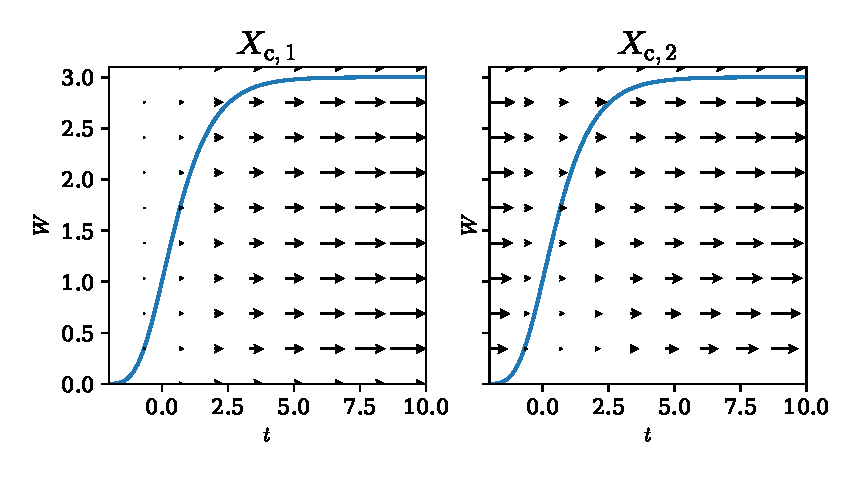
\includegraphics[width=.6517\textwidth]{images/gompertz-classical-local}
  \caption{
    The vector field of generators \(X_{\text{c},1}\) and \(X_{\text{c},2}\) superimposed on a solution curve.
    The \(\dl t\)- and \(\dl W\)-components of the vector fields are shown on a \(\log(1 + x)\) scale.
  }
  \label{fig:gompertz-classical-local}
\end{figure}
A representative of the only remaining transformation group, corresponding to \(X_{\text{c},3}\), is shown in \cref{fig:gompertz-classical-ansatz}.
\begin{figure}
  \centering
  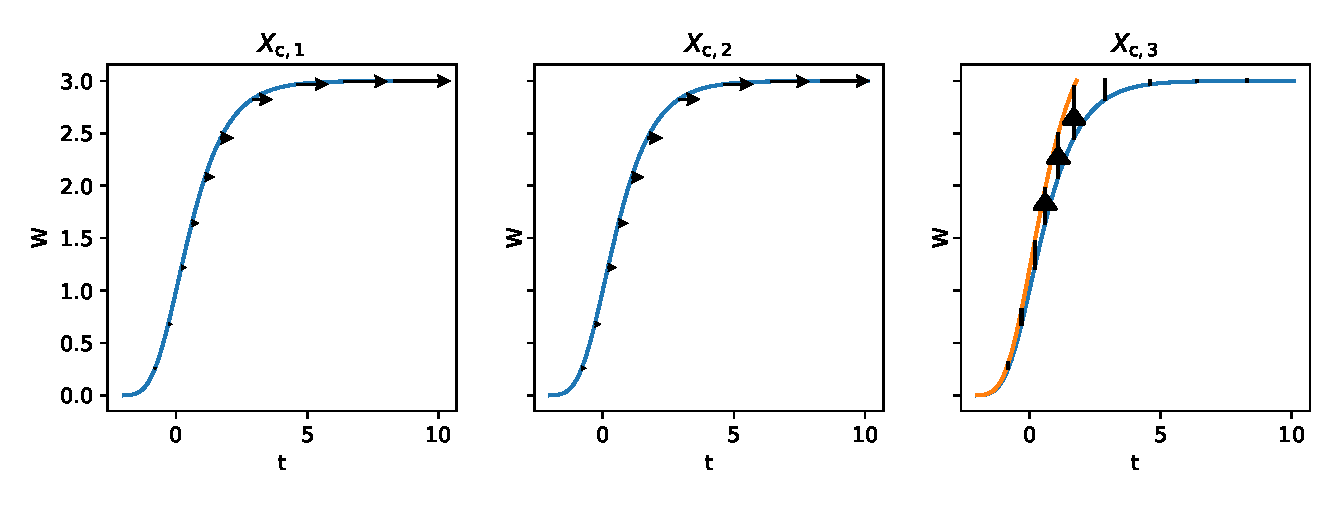
\includegraphics[width=.3355\textwidth]{images/gompertz-classical-ansatz}
  \caption{
    A representative transformation of the Lie group corresponding to the only non-trivial non-local symmetry generator of the classical Gompertz model found using an ansatz.
  }
  \label{fig:gompertz-classical-ansatz}
\end{figure}

\subsection{The autonomous Gompertz model}

The ansatz
\begin{align*}
  \xi(t, W) &= f_1(t) + f_2(t) \ln\left(\frac{W}{A}\right),\\
  \eta(t, W) &= f_3(t) W + f_4(t) \ln\left(\frac{W}{A}\right) W
\end{align*}
can be taken, where \(f_i\) for \(i =1,2,3,4\) are arbitrary functions in \(t\).
This results in the determining equation
\begin{align*}
  f_3'(t) W &+ f_4'(t) \ln\left(\frac{W}{A}\right) W \\
  &+ \left( f_3(t) + f_4(t) \left( 1 + \ln\left(\frac{W}{A}\right) \right) - \left( f_1'(t) + f_2'(t) \ln\left(\frac{W}{A}\right) \right) \right) \cdot -k_G \ln\left(\frac{W}{A}\right) W \\
  &- \frac{f_2(t)}{W} \left( k_G \ln\left(\frac{W}{A}\right) W \right)^2 =\\
  &= \left( f_3(t) W + f_4(t) \ln\left(\frac{W}{A}\right) W \right) \cdot -k_G \left( 1 + \ln\left(\frac{W}{A}\right) \right)
\end{align*}
which can be reduced to
\begin{align*}
  f_3'(t) W &+ \left( f_4'(t) + k_G f_1'(t) \right) \ln\left(\frac{W}{A}\right) W + \left( f_2'(t) - k_G f_2(t) \right) k_G \ln\left(\frac{W}{A}\right)^2 W =\\
  &= - k_G f_3(t) W
\end{align*}
By separating the equation based on powers of \(\ln\left(\frac{W}{A}\right)\), the system
\begin{subequations}
  \begin{flalign}
    W & : & f_3'(t) &= -k_G f_3(t) &\label{eq:W}\\
    \ln\left(\frac{W}{A}\right) W & : & f_4'(t) + k_G f_1'(t) &= 0 &\label{eq:WA}\\
    k_G \ln\left(\frac{W}{A}\right)^2 W & : & f_2'(t) - k_G f_2(t) &= 0 &\label{eq:kW2A2W}
  \end{flalign}
\end{subequations}
can be acquired.
This system of equations has the solution
\begin{align*}
  \xi(t, W) &= f_1(t) + c_1 e^{k_G t} \ln\left(\frac{W}{A}\right),\\
  \eta(t, W) &= c_2 e^{-k_G t} W + \left( c_3 - k_G f_1(t) \right) \ln\left(\frac{W}{A}\right) W,
\end{align*}
where \(c_1\), \(c_2\) and \(c_3\) are arbitrary constants.
Thus, by separating the tangent field into terms with independent arbitrary elements, the infinitesimal generators
\begin{align*}
  X_{\text{a},1} &= e^{k_G t} \ln\left(\frac{W}{A}\right) \partial_t \\
  X_{\text{a},2} &= e^{-k_G t} W \partial_W \\
  X_{\text{a},3} &= \ln\left(\frac{W}{A}\right) W \partial_W \\
  X_{\text{a},f} &= f(t) \partial_t - k_G f(t) \ln\left(\frac{W}{A}\right) W \partial_W
\end{align*}
of Lie point symmetries of the autonomous Gompertz ODE \labelcref{eq:gompertz-autonomous} are found.
The corresponding transformations can be seen in \cref{fig:gompertz-autonomous-ansatz}.
\begin{figure}
  \centering
  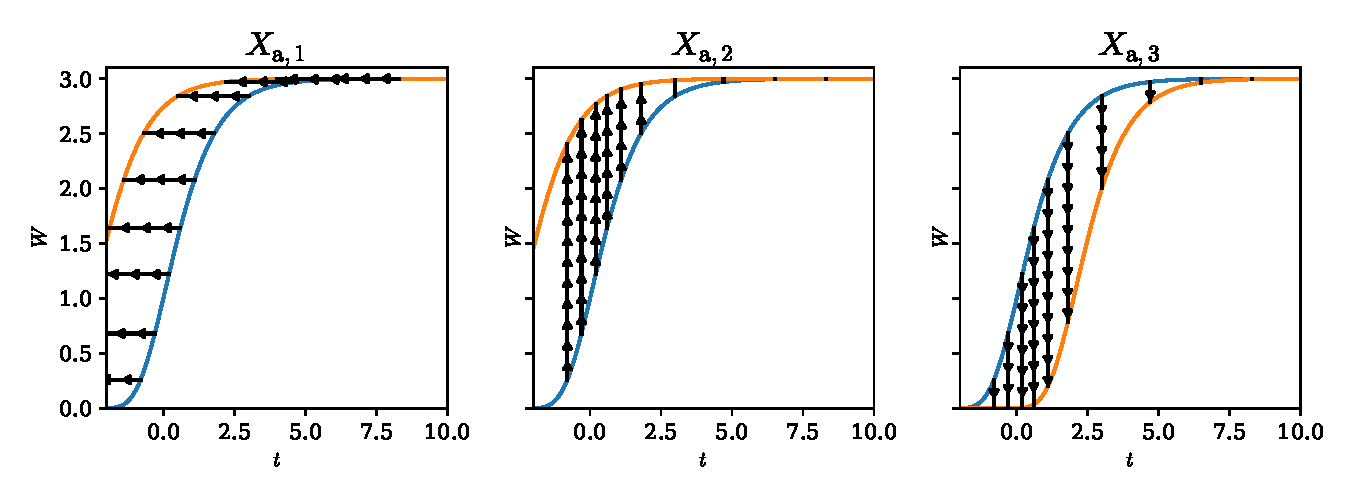
\includegraphics[width=.96\textwidth]{images/gompertz-autonomous-ansatz}
  \caption{Representative transformations of the Lie groups corresponding to symmetry generators of the autonomous Gompertz model found using an ansatz.}
  \label{fig:gompertz-autonomous-ansatz}
\end{figure}

\subsection{The system Gompertz model}

As models and ansätze grow in size, the determining equations grow.
This becomes particularly prominent for systems of ODE:s.
For this reason, the calculations for the remaining models in this chapter have been made using computer algebra using code outlined in \cref{app:computer-algebra}.

Similarly to the classical Gompertz model, the ansatz
\begin{align*}
  \xi{\left(t,W,G \right)} &= f_{1}{\left(t \right)} + f_{2}{\left(t \right)} W + f_{3}{\left(t \right)} G \\
  \eta^{1}{\left(t,W,G \right)} &= f_{4}{\left(t \right)} + f_{5}{\left(t \right)} W + f_{6}{\left(t \right)} G\\
  \eta^{2}{\left(t,W,G \right)} &= f_{7}{\left(t \right)} + f_{8}{\left(t \right)} W + f_{9}{\left(t \right)} G,
\end{align*}
where \(f_i\) are arbitrary functions in \(t\), is used.
The two determining equations can be decomposed in \(W\) and \(G\), resulting in 15 algebraic and ordinary differential equations.
By first solving the algebraic equations, followed by the differential for the arbitrary functions \(f_i\), their form can be determined resulting in the general form
\begin{align*}
  \xi{\left(t,W,G \right)} &= G c_{3} e^{k_{G} t} + c_{1} - \frac{c_{2} e^{k_{G} t}}{k_{G}} \\
  \eta^{1}{\left(t,W,G \right)} &= W c_{4} - \frac{W c_{5} e^{- k_{G} t}}{k_{G}} \\
  \eta^{2}{\left(t,W,G \right)} &= G c_{2} e^{k_{G} t} + c_{5} e^{- k_{G} t}.
\end{align*}
Decomposition in arbitrary constants result in the basis
\begin{align*}
  X_{\text{s},1} &= \partial_t \\
  X_{\text{s},2} &= - \frac{e^{k_{G} t}}{k_{G}} \partial_t + G e^{k_{G} t} \partial_G \\
  X_{\text{s},3} &= G e^{k_{G} t} \partial_t \\
  X_{\text{s},4} &= W \partial_W \\
  X_{\text{s},5} &= - \frac{W e^{- k_{G} t}}{k_{G}} \partial_W + e^{- k_{G} t} \partial_G.
\end{align*}
The corresponding transformations can be seen in \cref{fig:gompertz-system-ansatz}.
\begin{figure}
  \centering
  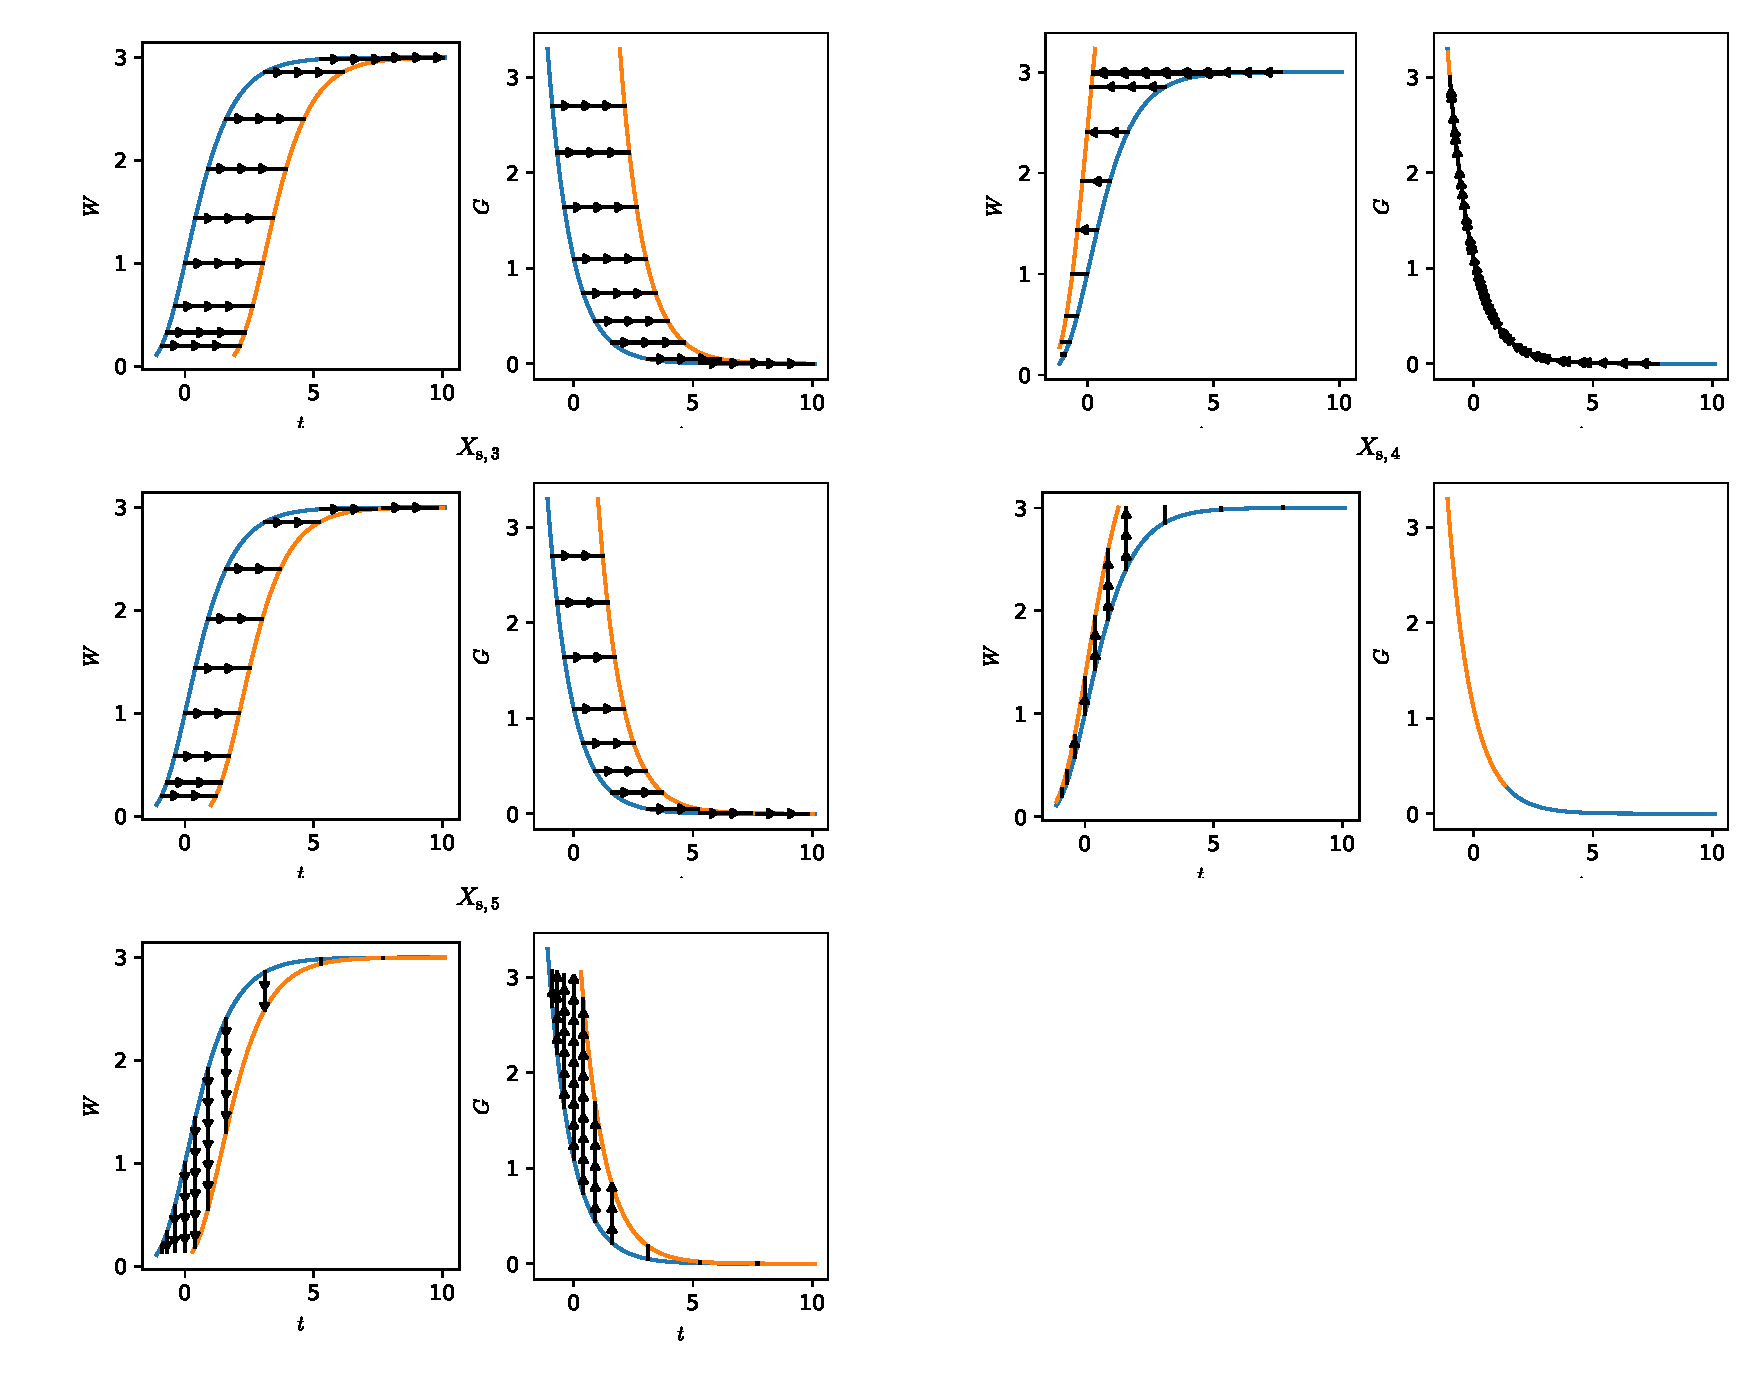
\includegraphics[width=.96\textwidth]{images/gompertz-system-ansatz}
  \caption{Representative transformations of the Lie groups corresponding to symmetry generators of the system Gompertz model found using an ansatz.}
  \label{fig:gompertz-system-ansatz}
\end{figure}

\section{The Lotka--Volterra model}

The Lotka--Volterra predator-prey model formulated in \cref{eq:lotka-volterra} has a right hand side formulated as second order polynomial in the two states \(N\) and \(P\).
A good starting point for ansätze is therefore polynomials, and arbitrary third degree polynomials in \(t\), \(N\) and \(P\) are chosen.
The ansatz will thus have the form
\begin{subequations} \label[subequations]{eq:lotka-volterra-ansatz}
  \begin{align}
    \xi &= c_{1,1} + c_{1,2}t + c_{1,3}N + c_{1,4}P + c_{1,5}t^{2} + c_{1,6}tN + c_{1,7}N^{2} + c_{1,8}tP + \\ & \qquad + c_{1,9}NP + c_{1,10}P^{2} + c_{1,11}t^{3} + c_{1,12}t^{2}N + c_{1,13}tN^{2} + c_{1,14}N^{3} + \\ & \qquad + c_{1,15}t^{2}P + c_{1,16}tNP + c_{1,17}N^{2}P + c_{1,18}tP^{2} + c_{1,19}NP^{2} + c_{1,20}P^{3} \\
    \eta^{1} &= c_{2,1} + c_{2,2}t + c_{2,3}N + c_{2,4}P + c_{2,5}t^{2} + c_{2,6}tN + c_{2,7}N^{2} + c_{2,8}tP + \\ & \qquad + c_{2,9}NP + c_{2,10}P^{2} + c_{2,11}t^{3} + c_{2,12}t^{2}N + c_{2,13}tN^{2} + c_{2,14}N^{3} + \\ & \qquad + c_{2,15}t^{2}P + c_{2,16}tNP + c_{2,17}N^{2}P + c_{2,18}tP^{2} + c_{2,19}NP^{2} + c_{2,20}P^{3} \\
    \eta^{2} &= c_{3,1} + c_{3,2}t + c_{3,3}N + c_{3,4}P + c_{3,5}t^{2} + c_{3,6}tN + c_{3,7}N^{2} + c_{3,8}tP + \\ & \qquad + c_{3,9}NP + c_{3,10}P^{2} + c_{3,11}t^{3} + c_{3,12}t^{2}N + c_{3,13}tN^{2} + c_{3,14}N^{3} + \\ & \qquad + c_{3,15}t^{2}P + c_{3,16}tNP + c_{3,17}N^{2}P + c_{3,18}tP^{2} + c_{3,19}NP^{2} + c_{3,20}P^{3},
  \end{align}
\end{subequations}
where \(c_{i,j}\) are arbitrary constants.
The linearized symmetry condition will thus consist of two equations, each of which must hold for arbitrary \(t\), \(N\) and \(P\).
The two equations can thus be decomposed into 98 linear equations in the arbitrary constants \(c_{i,j}\).
The solution to this overdetermined system of equations gives that any symmetry generator on the form of the ansatz can be written as a linear combination of the generators
\begin{align*}
  X_1 &= \partial_t \\
  X_2 &= \frac{-bNP + aN}{c} \partial_N + \frac{cNP - dP}{c} \partial_P \\
  X_3 &= \frac{t}{c} \partial_t + \frac{-btNP + atN}{c} \partial_N + \frac{ctNP - dtP}{c} \partial_P \\
  X_4 &= \frac{N}{c} \partial_t + \frac{-bcN^2P + acN^2 - bdNP + adN}{c^2} \partial_N + \frac{c^2N^2P - d^2P}{c^2} \partial_P \\
  X_5 &= \frac{P}{c} \partial_t + \frac{-bNP^2 + aNP}{c} \partial_N + \frac{cNP^2 - dP^2}{c} \partial_P
\end{align*}

\section{The Yildirim--Mackey lactose operon model} \label{sec:lac-operon-ansatze}

Since the lactose operon model formulated in \cref{eq:lac-operon} is significantly larger than all other models studied, the performance of the computer algebra system places restrictions on the ansätze viable to test.
Additionally, the decomposition of the linearized symmetry condition becomes less straight forward as the right hand side of the lactose operon model contains both fractions and arbitrary powers of the state \(A\).

A simple ansatz is that the infinitesimal generator is linear in time and the states, formulated as
\begin{align*}
  \xi &= c_{1,1} + c_{1,2}t + c_{1,3}M + c_{1,4}B + c_{1,5}L + c_{1,6}A + c_{1,7}P \\
  \eta^{1} &= c_{2,1} + c_{2,2}t + c_{2,3}M + c_{2,4}B + c_{2,5}L + c_{2,6}A + c_{2,7}P \\
  \eta^{2} &= c_{3,1} + c_{3,2}t + c_{3,3}M + c_{3,4}B + c_{3,5}L + c_{3,6}A + c_{3,7}P \\
  \eta^{3} &= c_{4,1} + c_{4,2}t + c_{4,3}M + c_{4,4}B + c_{4,5}L + c_{4,6}A + c_{4,7}P \\
  \eta^{4} &= c_{5,1} + c_{5,2}t + c_{5,3}M + c_{5,4}B + c_{5,5}L + c_{5,6}A + c_{5,7}P \\
  \eta^{5} &= c_{6,1} + c_{6,2}t + c_{6,3}M + c_{6,4}B + c_{6,5}L + c_{6,6}A + c_{6,7}P,
\end{align*}
where  \(c_{i,j}\) are arbitrary constants.
The linearized symmetry condition will thus consist of 5 equations, which will consist of sums of fractional expressions in the states.
To decompose the system, the sums in all equations are rewritten with a common denominator.
Additionally, since the power \(A^n\) appear in some of the equations, and all equations sought should hold for an arbitrary \(n\), the numerator of the equations written with common denominators is decomposed in \(t\), \(M\), \(B\), \(L\), \(A\), \(P\) and \(A^n\).
The decomposition results in 1901 equations, all linear in the arbitrary constants \(c_{i,j}\).
The solution to the overdetermined system of equations gives that the only symmetry generator on the form of the ansatz is the manifest generator
\begin{equation*}
  X_1 = \partial_t.
\end{equation*}
